% This is the Reed College LaTeX thesis template. Most of the work
% for the document class was done by Sam Noble (SN), as well as this
% template. Later comments etc. by Ben Salzberg (BTS). Additional
% restructuring and APA support by Jess Youngberg (JY).
% Your comments and suggestions are more than welcome; please email
% them to cus@reed.edu
%
% See https://www.reed.edu/cis/help/LaTeX/index.html for help. There are a
% great bunch of help pages there, with notes on
% getting started, bibtex, etc. Go there and read it if you're not
% already familiar with LaTeX.
%
% Any line that starts with a percent symbol is a comment.
% They won't show up in the document, and are useful for notes
% to yourself and explaining commands.
% Commenting also removes a line from the document;
% very handy for troubleshooting problems. -BTS

% As far as I know, this follows the requirements laid out in
% the 2002-2003 Senior Handbook. Ask a librarian to check the
% document before binding. -SN

%%
%% Preamble
%%
% \documentclass{<something>} must begin each LaTeX document
\documentclass[12pt,twoside]{reedthesis}
% Packages are extensions to the basic LaTeX functions. Whatever you
% want to typeset, there is probably a package out there for it.
% Chemistry (chemtex), screenplays, you name it.
% Check out CTAN to see: https://www.ctan.org/
%%
\usepackage{graphicx,latexsym}
\usepackage{amsmath}
\usepackage{amssymb,amsthm}
\usepackage{longtable,booktabs,setspace}
\usepackage{chemarr} %% Useful for one reaction arrow, useless if you're not a chem major
\usepackage[hyphens]{url}
% Added by CII
\usepackage{hyperref}
\usepackage{lmodern}
\usepackage{float}
\floatplacement{figure}{H}
% Thanks, @Xyv
\usepackage{calc}
% End of CII addition
\usepackage{rotating}

% Next line commented out by CII
%%% \usepackage{natbib}
% Comment out the natbib line above and uncomment the following two lines to use the new
% biblatex-chicago style, for Chicago A. Also make some changes at the end where the
% bibliography is included.
%\usepackage{biblatex-chicago}
%\bibliography{thesis}


% Added by CII (Thanks, Hadley!)
% Use ref for internal links
\renewcommand{\hyperref}[2][???]{\autoref{#1}}
\def\chapterautorefname{Chapter}
\def\sectionautorefname{Section}
\def\subsectionautorefname{Subsection}
% End of CII addition

% Added by CII
\usepackage{caption}
\captionsetup{width=5in}
% End of CII addition

% \usepackage{times} % other fonts are available like times, bookman, charter, palatino

% Syntax highlighting #22

% To pass between YAML and LaTeX the dollar signs are added by CII
\title{Computational analysis of multi-omics data to understand the molecular mechanisms of germline-dependent epigenetic inheritance}
\author{Deepak Kumar Tanwar}
% The month and year that you submit your FINAL draft TO THE LIBRARY (May or December)
\date{}
\division{}
\advisor{}
\institution{ETH Zurich}
\degree{}
%If you have two advisors for some reason, you can use the following
% Uncommented out by CII
% End of CII addition

%%% Remember to use the correct department!
\department{}
% if you're writing a thesis in an interdisciplinary major,
% uncomment the line below and change the text as appropriate.
% check the Senior Handbook if unsure.
%\thedivisionof{The Established Interdisciplinary Committee for}
% if you want the approval page to say "Approved for the Committee",
% uncomment the next line
%\approvedforthe{Committee}

% Added by CII
%%% Copied from knitr
%% maxwidth is the original width if it's less than linewidth
%% otherwise use linewidth (to make sure the graphics do not exceed the margin)
\makeatletter
\def\maxwidth{ %
  \ifdim\Gin@nat@width>\linewidth
    \linewidth
  \else
    \Gin@nat@width
  \fi
}
\makeatother

% From {rticles}

\renewcommand{\contentsname}{Table of Contents}
% End of CII addition

\setlength{\parskip}{0pt}

% Added by CII

\providecommand{\tightlist}{%
  \setlength{\itemsep}{0pt}\setlength{\parskip}{0pt}}

\Acknowledgements{
This doctoral thesis has been an accomplishment that would not have been possible, or anywhere near as enjoyable, without the help and support of a number of incredible individuals. Thank you for all that you have contributed to this thesis. \newline\newline I am eternally grateful to Prof.~Dr.~Isabelle Mansuy for allowing me to do Doctoral research in her lab. It is a pleasure to be a member of the Neuroepigenetics lab. Thank you to all the members of the Neuroepigenetics lab, past and present. The Neuroepigenetics group was always fun to work with and I learned a lot about experiments. Thank you so much! A special thanks to the present and past members of Y38 for motivating, and various scientific and non-scientific discussions. \newline\newline My sincere thanks to Prof.~Dr.~Mark Robinson and Prof.~Dr.~Tuncay Baubec for accepting to be my co-examiners and supporting me throughout my doctoral research. Thank you so much Mark for always being available and providing all the help in writing proposals, helping in supervising students, and discussing and providing solutions to the problems I was facing. \newline\newline I am indebted to Dr.~Pierre-Luc Germain for his expert supervision and all the support he has provided. I am grateful for all discussions and suggestions on both scientific and non-scientific issues. Thank you for being so nice and for all the support which was extremely helpful to reach this point. I have learnt a lot from you. \newline\newline I would also like to thank the Directors and members of the Brain Research Institute for creating such a stimulating environment for research. \newline\newline I am extremely grateful for my doctoral funding, the Swiss Government Excellence Scholarship. Thank you so much Sandra Zweifel for always being there. \newline\newline Looking back into the past, this thesis would not have happened without my bachelor's thesis supervisors Rainer König and Sandro Lindig, who got me interested in the field of bioinformatics data science. \newline\newline Finally, I am very grateful to my family for their continuous support and belief in me. Visiting you always helped me to relax and to not worry about work so much. Last of all, I want to thank my wife, Palni Kundra, for always cheering me up when I was down and for helping me with stupid issues.
}

\Dedication{

}

\Preface{

}

\Abstract{

}

	\usepackage{setspace}\onehalfspacing
 \usepackage{acronym}
 \usepackage{glossaries}
 \usepackage{biblatex}
 \usepackage{fancyhdr}
 \usepackage{graphics}
 \usepackage{float}
 \usepackage{lmodern}
 \usepackage{pdflscape}
 \usepackage{caption}
 \captionsetup{font=footnotesize}
 \usepackage[labelfont=bf]{caption}
 \usepackage{wrapfig}
 \usepackage{pdfpages}
 \usepackage{afterpage}
 \usepackage[section]{placeins}
	\usepackage{flafter}
 \usepackage{float}
 \usepackage{subfig}
 \usepackage{subfloat}
 \usepackage{booktabs}
 \usepackage{longtable}
 \usepackage{array}
 \usepackage{multirow}
 \usepackage{wrapfig}
 \usepackage{colortbl}
 \usepackage{pdflscape}
 \usepackage{tabu}
 \usepackage{threeparttable}
 \usepackage{threeparttablex}
 \usepackage[normalem]{ulem}
 \usepackage{makecell}
 \usepackage{xcolor}
% End of CII addition
%%
%% End Preamble
%%
%
\begin{document}

% Everything below added by CII
  \maketitle

\frontmatter % this stuff will be roman-numbered
\pagestyle{empty} % this removes page numbers from the frontmatter
  \begin{acknowledgements}
    This doctoral thesis has been an accomplishment that would not have been possible, or anywhere near as enjoyable, without the help and support of a number of incredible individuals. Thank you for all that you have contributed to this thesis. \newline\newline I am eternally grateful to Prof.~Dr.~Isabelle Mansuy for allowing me to do Doctoral research in her lab. It is a pleasure to be a member of the Neuroepigenetics lab. Thank you to all the members of the Neuroepigenetics lab, past and present. The Neuroepigenetics group was always fun to work with and I learned a lot about experiments. Thank you so much! A special thanks to the present and past members of Y38 for motivating, and various scientific and non-scientific discussions. \newline\newline My sincere thanks to Prof.~Dr.~Mark Robinson and Prof.~Dr.~Tuncay Baubec for accepting to be my co-examiners and supporting me throughout my doctoral research. Thank you so much Mark for always being available and providing all the help in writing proposals, helping in supervising students, and discussing and providing solutions to the problems I was facing. \newline\newline I am indebted to Dr.~Pierre-Luc Germain for his expert supervision and all the support he has provided. I am grateful for all discussions and suggestions on both scientific and non-scientific issues. Thank you for being so nice and for all the support which was extremely helpful to reach this point. I have learnt a lot from you. \newline\newline I would also like to thank the Directors and members of the Brain Research Institute for creating such a stimulating environment for research. \newline\newline I am extremely grateful for my doctoral funding, the Swiss Government Excellence Scholarship. Thank you so much Sandra Zweifel for always being there. \newline\newline Looking back into the past, this thesis would not have happened without my bachelor's thesis supervisors Rainer König and Sandro Lindig, who got me interested in the field of bioinformatics data science. \newline\newline Finally, I am very grateful to my family for their continuous support and belief in me. Visiting you always helped me to relax and to not worry about work so much. Last of all, I want to thank my wife, Palni Kundra, for always cheering me up when I was down and for helping me with stupid issues.
  \end{acknowledgements}

  \hypersetup{linkcolor=black}
  \setcounter{secnumdepth}{4}
  \setcounter{tocdepth}{4}
  \tableofcontents

  \listoftables

  \listoffigures



\mainmatter % here the regular arabic numbering starts
\pagestyle{fancyplain} % turns page numbering back on

\hypertarget{ae}{%
\chapter*{Appendix E}\label{ae}}
\addcontentsline{toc}{chapter}{Appendix E}

Curriculum Vitae of the doctoral student.

\setcounter{secnumdepth}{-1}
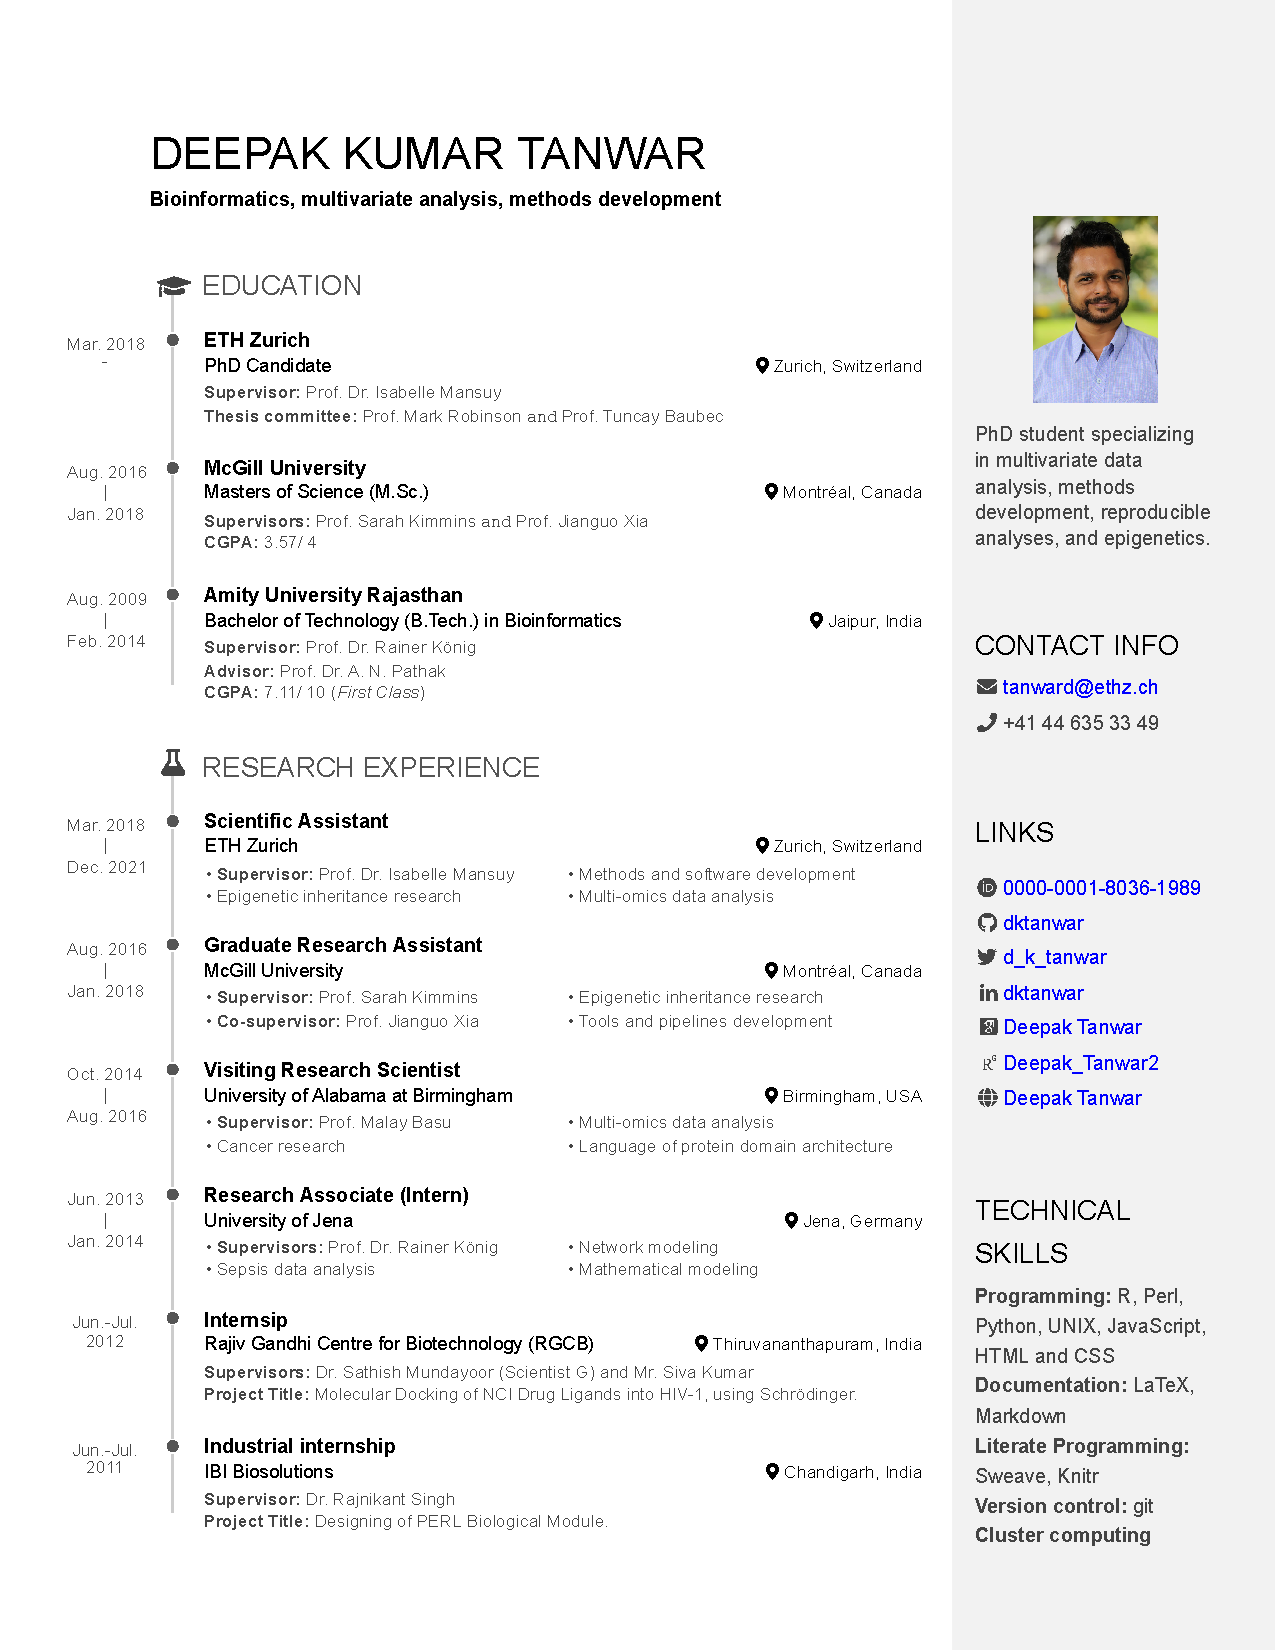
\includepdf[pages=-,addtotoc={1, section, 1, CV, CV}]{data/Deepak_Tanwar.pdf}

\backmatter

\hypertarget{references}{%
\chapter*{References}\label{references}}
\addcontentsline{toc}{chapter}{References}

\markboth{References}{References}

\noindent

\setlength{\parindent}{-0.20in}


% Index?

\end{document}
\newpage

Dedicated to
